\documentclass[a4paper,12pt]{article}
\usepackage[margin=0.8 in]{geometry}

\usepackage[T2A]{fontenc}			% кодировка
\usepackage[utf8]{inputenc}			% кодировка исходного текста
\usepackage[english,russian]{babel}	% локализация и переносы
\usepackage{graphicx}                % Математика
\usepackage{amsmath,amsfonts,amssymb,amsthm,mathtools} 
\usepackage{mathtext}
\usepackage[T2A]{fontenc}
\usepackage[utf8]{inputenc}

\usepackage{wasysym}

\usepackage{placeins}

%Заговолок
\author{Бичина Марина 
группа Б04-005 1 курса ФЭФМ}
\title{}
\date{}


\begin{document} % начало документа

\begin{center}
\begin{Large}
{Бичина Марина Б04-005, Лабораторная работа №.3.5.1}
\end{Large}
\end{center}
\paragraph{Цель работы:} 
\begin{enumerate}
\itemsep0em
\item Измерить вольт-амперную тлеющего характеристику тлеющего разряда 
\item Измерить зондовые характеристики при разных токах разряда и изучить таким образом свойства плазмы (концентрацию и температуру электронов в плазме, степень ионизации,  плазменную частоту и дебаевский радиус экранирования)
\end{enumerate}
\paragraph{Оборудование:}
\begin{enumerate}
\itemsep0em
\item Стеклянная газоразрядная трубка, наполненная неоном
\item Высоковольтный источник питания 
\item Источник питания постоянного тока
\item Делитель напряжения
\item Потенциометр
\item Амперметры
\item Вольтметры
\item Переключатели
\end{enumerate}


\paragraph{Теоретическая справка:}
\paragraph{}
Плазмой называют ионизированный газ, дебаевский радиус которого $r_d$ во много раз меньше характерного размера объема, занимаемого этим газом \\
Дебаевский радиус - характерная длина, с которой с расстоянием экспоненциально убывает поле иона вследствие экранирующего действия
\begin{equation}
r_{D} = \sqrt{\frac{kT_{e}}{4\pi n e^2}}=743\sqrt{\frac{T_{e}}{n}}
\end{equation}
так же его можно определить как амплитуду ленгмюровских колебаний плазмы, возбуждаемых тепловыми флуктуациями. \\
Число частиц в дебаевской сфере - число частиц, много больших единицы, для которых потенциальная энергия взаимодействия 2 заряженных частиц существенно меньше тепловой энергии. Их число примерно равно
\begin{equation*}
N_{D}\approx n\cdot \frac{4}{3}\pi r^3_{D} \approx 0.1\frac{1}{e^3}\sqrt{\frac{kT_e^3}{n}}
\end{equation*}
Плазменная частота - время отклика на флуктуацию плотности заряда в плазме
\begin{equation}
\omega_{p} = \frac{4\pi ne^2}{m} = 5.65\cdot 10^4 \sqrt{n} \;\;\;=>\;\;\; r_{D} = \frac{\vartheta}{\omega_{p}}
\end{equation}
Температура электронов в энергетических единицах
\begin{equation}
k_\text{Б}T_e = \frac{1}{2}\frac{eI_{\text{iн}}}{\frac{dI}{dU}|_{U=0}}
\end{equation}
Концентрация заряженных частиц:
\begin{equation}
n_i = \frac{I}{0.4eS}\sqrt{\frac{m_i}{2k_{\text{Б}}T_e}}
\end{equation}
\paragraph{Описание установки:}
\paragraph{}
\begin{center}
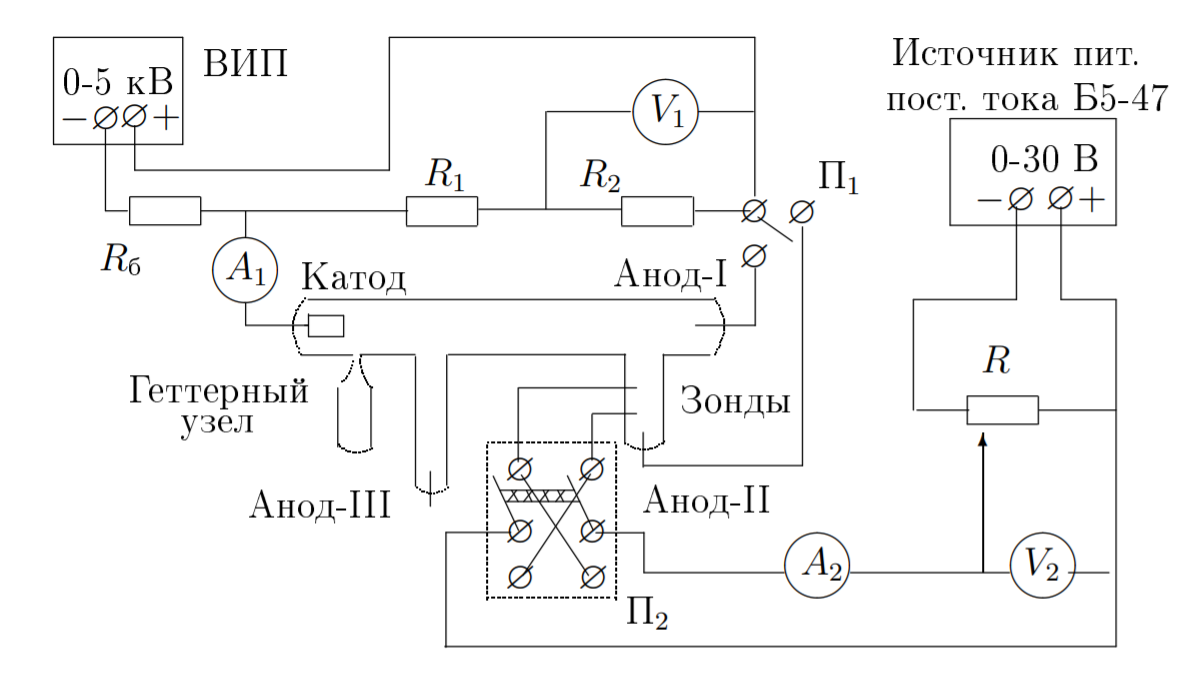
\includegraphics[scale=0.55]{setup.png}
\end{center}
\setlength{\parindent}{1.5 cm}
	Стеклянная газоразрядная трубка имеет холодный полый катод, три анода и \textit{геттерный} узел. Трубка наполнена изотопом неона $^2_2$Ne при давлении 2 мм рт. ст. Катод и один из анодов (I и II) с помощью переключателя $\Pi_1$ подключается через балластный резистор $R_\text{б}$ ($\approx 450$ кОм) к регулируемому ВИП с выходным напряжением до 5 кВ.\\
	Зонды изготовлены из молибденовой проволоки диаметром $d = 0.2$ мм и имеют длину $l = 5.2$ мм.

\paragraph{Ход работы:}
\begin{enumerate}
\itemsep0em
\item Рассмотрим ВАХ разряда: для этого по снятым данным построим график
\begin{figure}[h!]
\centering
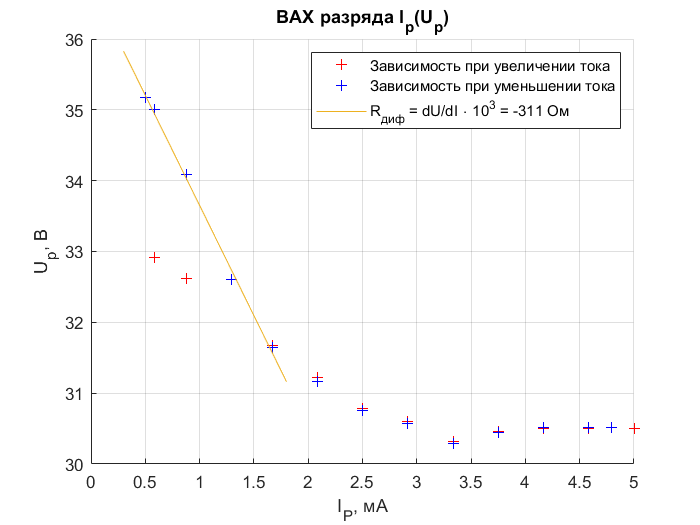
\includegraphics[scale=0.7]{graph_r.png}
\label{razr}
\caption{}
\end{figure}\\
 Далее по наклону прямой найдем максимальное дифференциальное  сопротивление разряда, получим $\dfrac{dU}{dI} = -310 \pm 10 \;\;\text{Ом}$\\
 Так же, мы можем сравнить полученных выше график с вольт-амперной характеристикой разряда в неоне. Построим график в логарифмических координатах
 \begin{figure}[h!]
 \centering
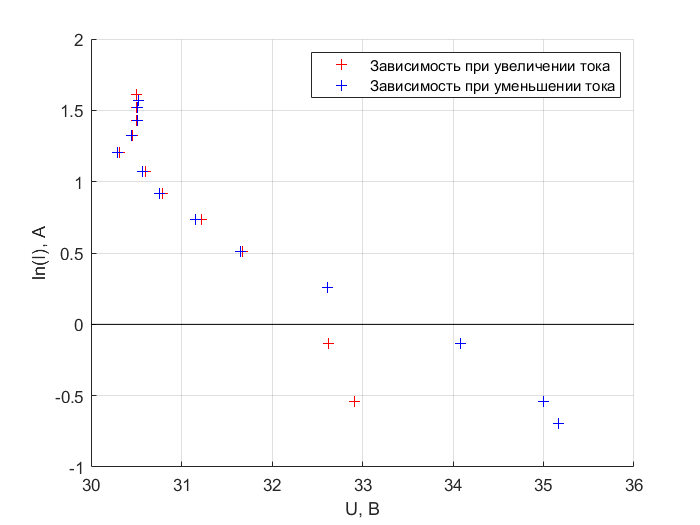
\includegraphics[scale=0.7]{graph_r_log.png}
\label{razr_log}
\caption{}
\end{figure}
Можно заметить, что значение сопротивления у нас вышло отрицательным. Здесь нет ошибки. \\
 Дифференциальное сопротивление может быть отрицательным, поскольку возрастание тока приводит к возрастанию концентрации ионов, из-за чего возрастает проводимость и понижается напряжение\\
Сам график соответствует промежутку Д-Г
\FloatBarrier
\item Зондовые характеристики\\
Обработка графиков будет производится в виде:
 \begin{figure}[h!]
 \centering
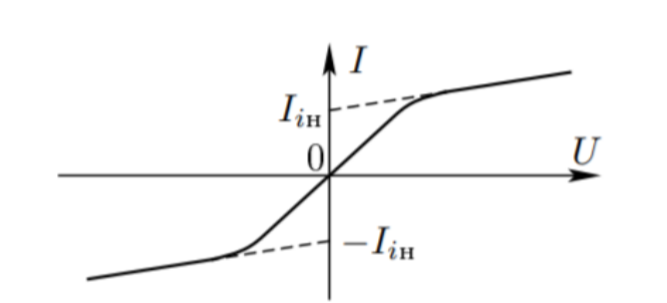
\includegraphics[scale=0.6]{vid.png}
\caption{ВАХ двойного зонда}
\end{figure}

\FloatBarrier 
\begin{figure}[h!]
\centering
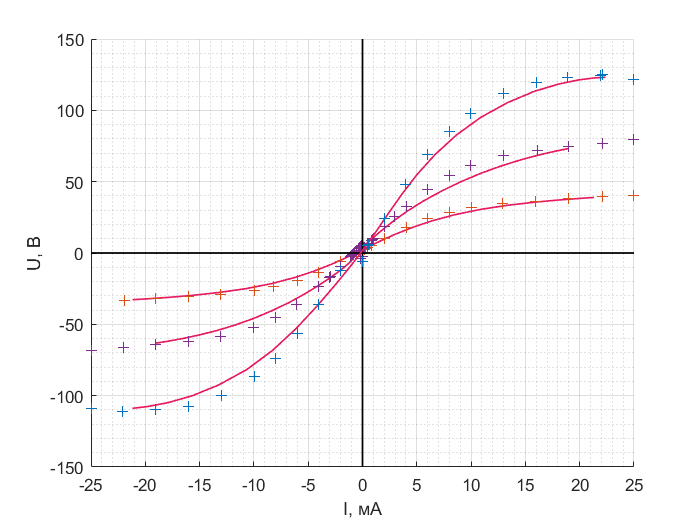
\includegraphics[scale=0.6]{graph_sum.png}
\caption{семейство вольт-амперных характеристик двойного зонда $I_{\text{з}}(U_{\text{з}})$, с постоянным током разряда в диапазоне от 1.5 до 5 мА}
\end{figure}
Ионный ток насыщения $I_{\text{iн}}$ мы можем определить, проведя прямые по МНК: y = ax + b, где коэффициент $b = I_{\text{iн}}$ (на графиках соответствует уравнению 1) \\
Величину $\Delta U$ мы можем определить по графику 2, подставляя $y=I_{\text{iн}}$ ($\Delta U$ соответствует значению х в данном уравнении)
\begin{figure}[h!]
\centering
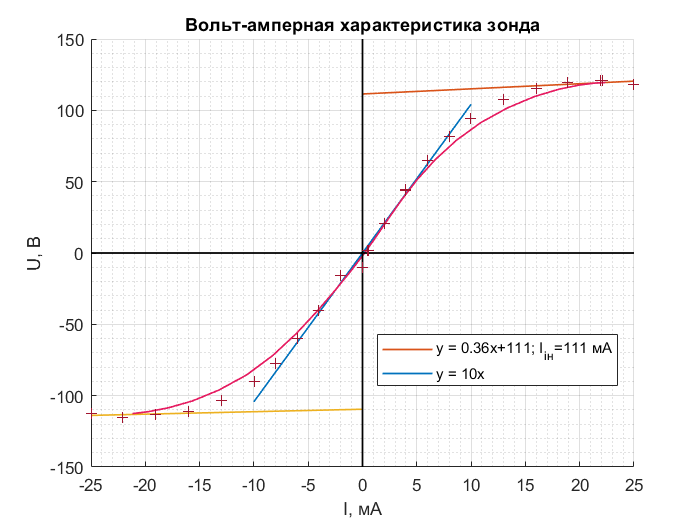
\includegraphics[scale=0.6]{graph_1_1.png}
\caption{ВАХ двойного зонда $I_{\text{з}}(U_{\text{з}})$ для тока разряда $I_p = 4.8$ мА}
\end{figure}
\begin{figure}[h!]
\centering
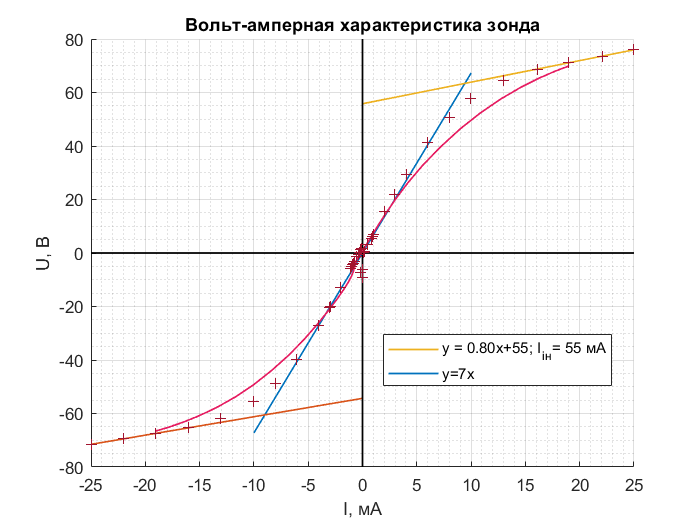
\includegraphics[scale=0.6]{graph_2_2.png}
\caption{ВАХ двойного зонда $I_{\text{з}}(U_{\text{з}})$ для тока разряда $I_p = 3$ мА}
\end{figure}
\begin{figure}[h!]
\centering
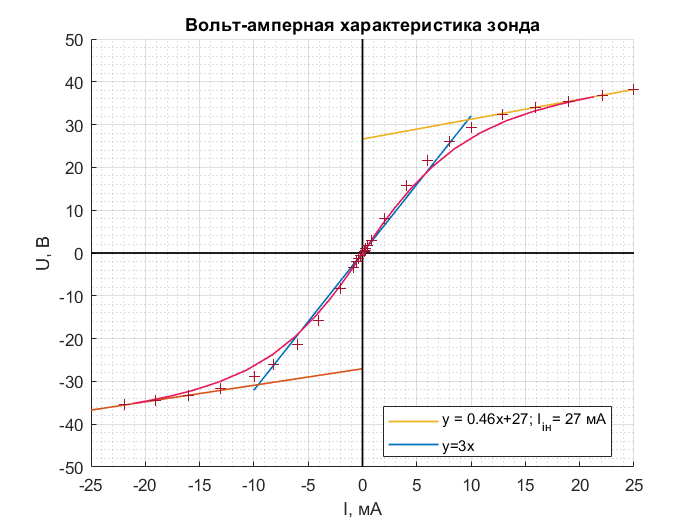
\includegraphics[scale=0.6]{graph_3_3.png}
\caption{ВАХ двойного зонда $I_{\text{з}}(U_{\text{з}})$ для тока разряда $I_p = 1.5$ мА}
\end{figure}
\item по данным из графиков построим таблицу для $I_p, I_{\text{iн}},\Delta U$ и их погрешностей:\\
\begin{table}[h!]
\centering
\begin{tabular}{|l||l|l|l|}
\hline
$I_p$, дел              & 120  & 75   & 37.5 \\ \hline
$I_p$ мА                & 4.8  & 3    & 1.5  \\ \hline
$I_{\text{iн}}$ мА      & 111  & 55   & 27   \\ \hline
$\sigma_{\text{iн}}$ мА & 4.62 & 1.22 & 0.28 \\ \hline
$\Delta U$, B           & 11.1 & 7.86 & 9    \\ \hline
$\sigma_{\Delta U}$, B  & 0.65 & 0.38 & 0.15 \\ \hline
\end{tabular}
\caption{Сводная таблица ВАХ двойного зонда для токов разряда 4.8-1.5 мА}
\end{table}
\item Рассчитаем температуру электронов и концентрацию заряженных частиц по формулам (3) и (4) соответственно
\[k_{\text{Б}}T_{e_1} = \frac{1}{2}\frac{eI_{\text{iн}}}{\frac{dI}{dU}|_{U=0}} = \frac{1}{2}\Delta U = \frac{11.1}{2} = 5.55 \;\; \text{эВ}\]
\[k_{\text{Б}}T_{e_2} = 3.93 \;\; \text{эВ}\]
\[k_{\text{Б}}T_{e_3} = 4.5 \;\; \text{эВ}\]

\[n_{i_1}=\frac{I}{0.4eS}\sqrt{\frac{m_i}{2k_\text{Б}T_e}}=6.9\cdot 10^{16}\text{м}^{-3}\]
\[n_{i_2}=4.57\cdot 10^{16}\text{м}^{-3}\]
\[n_{i_3}=2.30\cdot 10^{16}\text{м}^{-3}\]
\item Построим графики зависимостей электронной температуры и концентрации электронов от тока разряда $T_e(I_p), n_e(I_p)$
\begin{table}[h!]
\centering
\begin{tabular}{|l|l|l|l|}
\hline
$I_p$ мА              & 4.8  & 3    & 1.5 \\ \hline
$k_{\text{Б}}T_e$, эВ & 5.55 & 3.93 & 4.5 \\ \hline
\end{tabular}
\end{table}\\
\begin{figure}[h!]
\centering
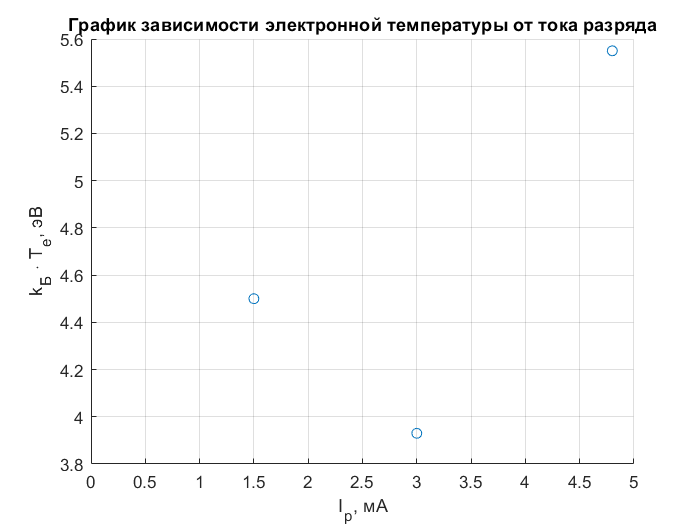
\includegraphics[scale=0.6]{graph_4.png}
\caption{}
\end{figure}
Видим, что мы не можем установить никакой зависимости температуры от тока разряда\\

\FloatBarrier 
\begin{table}[h!]
\centering
\begin{tabular}{|l|l|l|l|}
\hline
$I_p$ мА            & 4.8 & 3    & 1.5  \\ \hline
$n_i \cdot 10^{16}$ & 6.8 & 4.57 & 2.30 \\ \hline
\end{tabular}
\end{table}
\begin{figure}[h!]
\centering
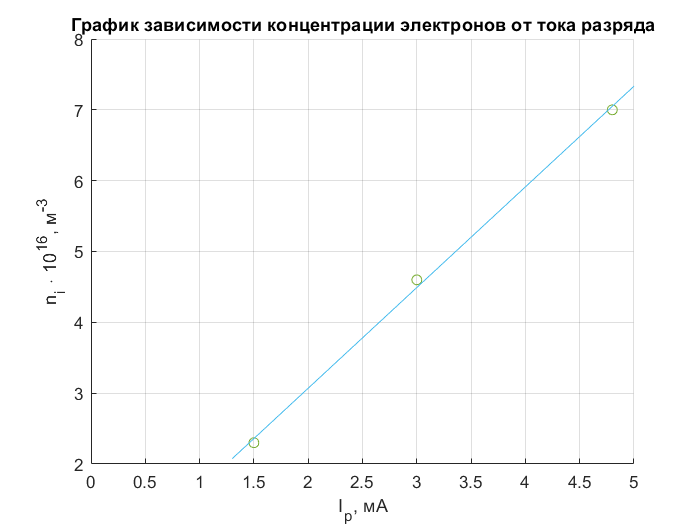
\includegraphics[scale=0.6]{graph_5.png}
\caption{}
\end{figure}
В данном случае мы можем обнаружить линейную зависимость
\item Рассчитаем плазменную частоту $\omega_p$, электронную поляризационную длину $r_De$ и дебаевский радиус экранирования $r_D$ по формулам (2) и (1). Результаты занесем в сводную таблицу:
\begin{table}[h!]
\centering
\begin{tabular}{|l||l|l|l|}
\hline
$n_i \cdot 10^{16}$                    & 6.8  & 4.57 & 2.30 \\ \hline
$\omega _p, \cdot 10^{13} \;\; c^{-1}$ & 1.48 & 1.20 & 0.85 \\ \hline
$r_{De}\;\;$см                         & 5.6  & 7    & 9.3  \\ \hline
$r_D\;\;$см                            & 0.43 & 0.53 & 0.74 \\ \hline
\end{tabular}
\end{table}
\end{enumerate}

\paragraph{Выводы:}
\begin{enumerate}
\item Мы измерили ВАХ тлеющего разряда. Получили значение дифференциальное сопротивление разряда, равное $R=-310 \pm 10$ Ом.
\item При исследовании графика зависимости установили, что наш диапазон соответствует участку Д-Г
\item Исследовали зондовые характеристики при разных токах разряда. Все данные представлены в сводной таблице:
\begin{table}[h!]
\centering
\begin{tabular}{|l|l|l|l|l|l|l|l|}
\hline
$I_p,$ мА & $I_{{\text{iн}}},$ мА & $\Delta U,$ B & $k_{\text{Б}}T_e$, эВ & $n_i \cdot 10^{16}$ & $\omega , c^{-1}\cdot 10^{13}$ & $r_{De}$, см & $r_D$, см      \\ \hline
4.8       & 111                 & 11.1          & $55.0 \pm 3.6$         & $6.8\pm 0.5$        & $1.5\pm 0.1$                    & $5.6\pm 0.6$ & $0.43\pm 0.03$ \\ \hline
3         & 55                  & 7.86          & $3.93\pm 2$            & $4.57\pm 0.20$      & $1.20\pm 0.05$                  & $7\pm 0.4$   & $0.53\pm 0.02$ \\ \hline
1.5       & 27                  & 9             & $4.5.0\pm 1.3$         & $2.30\pm 0.04$      & $0.85\pm 0.01$                  & $9.3\pm 0.2$ & $0.74\pm 0.01$ \\ \hline
\end{tabular}
\end{table}
\item Увидели, что для снятых нами данных какая-либо зависимость температуры от тока не обнаруживается
\item Обнаружили линейную зависимость концентрации от тока
\end{enumerate}
\end{document}